\begin{frame}
\frametitle{Autres analyses run 1}
\begin{columns}
\begin{column}{0.64\textwidth}
\begin{small}
\begin{maliste}
\item CMS (JHEP 11 (2014) 154) 
\begin{itemize}
\item 1 lepton, $\geq 6$ jets, $\geq 2$ b-jets
\item $H_T>400$~GeV, $E_T^\text{miss} > 30$~GeV
\item Interpr\'etation fr\'equentiste, fit BDT 
\end{itemize}
\vspace*{0.3cm}
\item ATLAS (JHEP 08 (2015) 105)
\begin{itemize}
\item 1 lepton, $\geq 5$ jets, $\geq 2$ b-jets, $E_T^\text{miss} \geq 20$~GeV
\item 8 r\'egions de signal
\item Interpr\'etation fr\'equentiste, fit $H_T$ 
\end{itemize}
\end{maliste}
\end{small}
\end{column}
\begin{column}{0.4\textwidth}
\begin{center}
\vspace*{-1.5cm}
\hspace*{-.4cm}
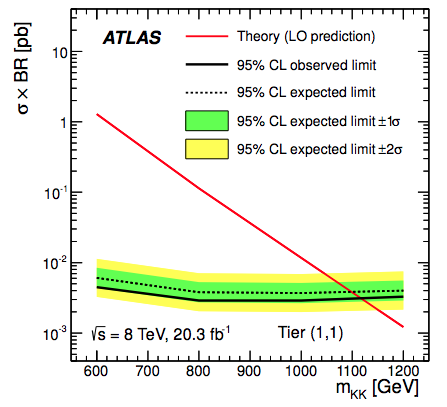
\includegraphics[width=0.89\textwidth]{Figures/FourTops/ATLASSingleLeptonResultTier11sym.png}
\\
%\vspace*{0.2cm}
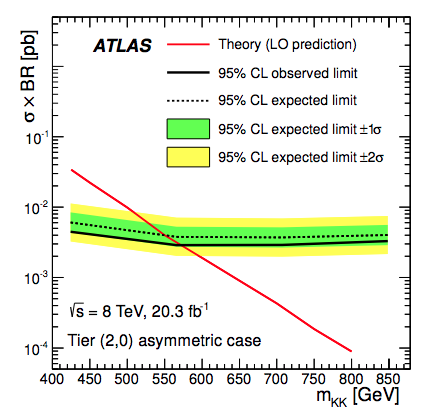
\includegraphics[width=0.86\textwidth]{Figures/FourTops/ATLASSingleLeptonResultTier20asym.png}
\end{center}
\end{column}
\end{columns}

\begin{scriptsize}
\begin{table}[htb]
  \begin{center}
\hspace*{-0.5cm}
    \begin{tabular}{|c|c|c|c|}
      \cline{2-4}
\multicolumn{1}{c|}{}   & ATLAS multilepton & ATLAS lepton+jets  & CMS lepton+jets \\ \hline
Modèle standard     & $70$~fb ($27$~fb)  & $23~$fb ($32$~fb) & $32$~fb ($32$~fb)\\ \hline
Interaction contact & $61$~fb ($22$~fb)  & $12~$fb ($16$~fb) & \multicolumn{1}{|c}{}\\ \cline{1-3}
2UED/RPP            & $m_{KK}>0.96~$TeV ($1.05$~TeV) & $m_{KK}>1.12~$TeV ($1.10$~TeV) & \multicolumn{1}{|c}{}\\ \cline{1-3}
    \end{tabular}
 \end{center}
\end{table}
\end{scriptsize}
\end{frame}
